\section{Theory}
\begin{figure*}
    \centering
    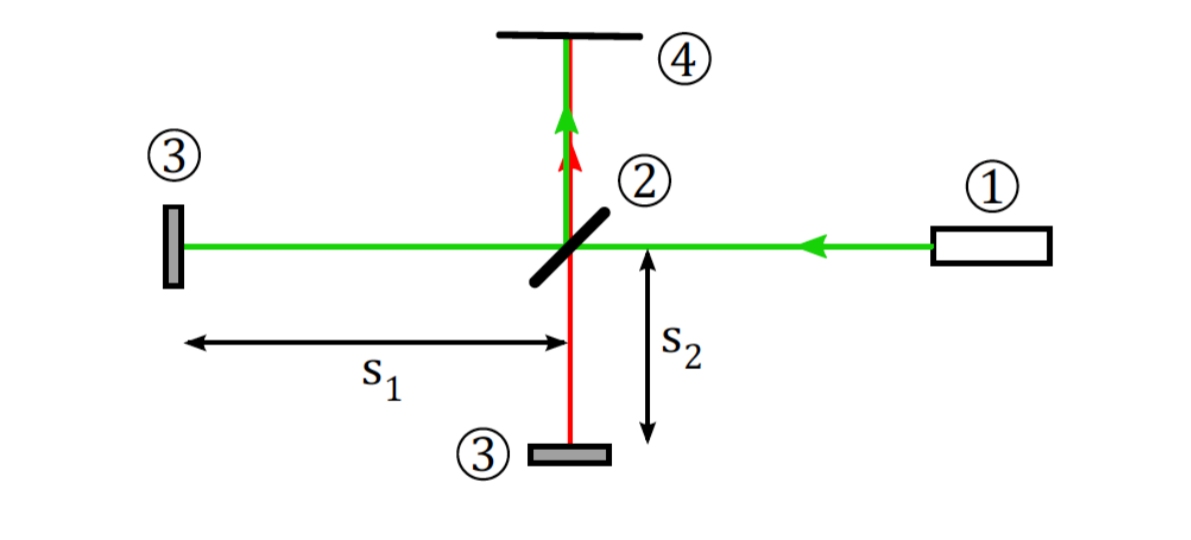
\includegraphics[width=\textwidth]{michelsonsetup}
    \caption{The simplest setup of a Michelson interferometer.}
    \label{fig:configuration}
\end{figure*}
\subsection{Michelson Interferometer}
A Michelson interferometer consist of atleast two mirrors, $m1$ and $m2$, and a beam splitter $m$. A light source $S$ emits light, which is split at the surface of $m$. As $m$ is partially reflective (in our experiment it is assumed to be $50/50$) This ensures that the light is transmitted and reflected equally at the surface of the beamsplitter.

A Michelson interferometer provies a powerful method of measuring the optical properties of a medium. By examining the fringes at the output of a Michelson interferometer one can yield the amplitudes and relative phases of the two beams traversing through reference arm and sample respectively. This holds the information of the optical properties of the medium placed in the sample. The fringes are generated by periodically varying the path length difference between the two arms. This can be done by using a piezo element to oscillate the position of the reference mirror. The mirror oscilattion varies the phase difference between the two beams, often refered to as phase modulation of the instrument.
\subsection{Interference}
\subsection{}<++>

\subsection{Piezo Electric Crystal}
%\fxme{Driven frequency, is it a resonance? Maximal displacement?}


